\documentclass{article}
\usepackage[utf8]{inputenc}
\usepackage{amsmath, amssymb}
\usepackage{float}
\usepackage{hyperref}
\usepackage[numbers,sort&compress]{natbib}
\usepackage{booktabs}
\usepackage{graphicx}
\usepackage{algorithm}
\usepackage{algpseudocode}

\title{Project Report on Symbolic Regression}
\author{Mher Mnatsakanyan}
\date{\today}

\begin{document}
\maketitle

\section{Introduction}

Symbolic regression searches for an actual mathematical formula that
explains given data, instead of fitting a black-box model to it. Our
interest in this is extrapolation. Models such as polynomials, random
forests or neural networks fit the training points well, but outside the
training interval they behave according to their model class rather than
according to the data. A formula behaves differently. If the points were
really produced by $f(x) = 0.5\,x \sin x + 0.1\,x^2$ and we recover this
formula, the predictions stay correct arbitrarily far from the training
points, though this only helps when the data actually follows a formula.

We study the effect on synthetic data. A generator samples random
formulas by drawing operators at random and produces a dataset from each
one, with noisy training points inside an interval and clean test points
outside it, so the test error measures extrapolation directly. Three
regressors then search for a formula: a hill climb guided by
Chatterjee's rank correlation coefficient $\xi$, classic genetic
programming via the \texttt{gplearn} library, and a small neural network
pretrained on generated data to predict formulas directly. We compare
them on a suite of test functions and probe their weaknesses with sweeps
over noise level, extrapolation distance and training set size.

\section{Three approaches to finding a formula}

All three regressors work on expression trees. Leaves are the input
variable $x$ or numeric constants, inner nodes are operators from
$\mathcal{O}_1 = \{\sin, \cos, \exp, \log, \sqrt{\cdot}\,, (\cdot)^2, -(\cdot)\}$
(one child) or $\mathcal{O}_2 = \{+, -, \times, \div\}$ (two children). A
tree $g$ defines a function $g(x)$, and its complexity $|g|$ is its
number of nodes. Regressors A and C use all of $\mathcal{O}_1$ and draw
constants from $[-2,2]$, while the \texttt{gplearn} operator set has
neither squaring nor negation and draws from $[-1,1]$. Given noisy
training data $(x_i, y_i)_{i=1}^n$ from an interval, each regressor must
return a function that also predicts well outside it. Regressors A and C
finish the same way. Once a promising structure is found, its numeric
constants and an outer rescaling $a\,g(x)+b$ are fitted with least
squares, since getting the constants right is essential for accurate
symbolic regression \citep{cranmer2023interpretablemachinelearningscience}. Regressor B is used as \texttt{gplearn}
returns it, without any constant fit, which is the source of the bias
discussed in Section~2.2.

\subsection{Regressor A: $\xi$-guided search}

The first regressor is a hill climb over trees. What distinguishes it is
a cheap test that rates a candidate before any fitting, Chatterjee's
correlation coefficient \citep{chatterjee2020newcoefficientcorrelation}. Sort the data by the
candidate's values $g(x_i)$ and walk through the corresponding $y$. If
$y$ really is a function of $g$, neighbouring $y$ change smoothly and
their ranks barely move from one point to the next, whereas if $g$ has
nothing to do with $y$ the ranks jump around at random. The coefficient
$\xi_n(g, y)$ turns the total size of those jumps into a number near $1$
in the first case and near $0$ in the second. Because it only uses
ranks, it costs $O(n \log n)$ with no fitting involved, is insensitive
to the scale of $g$, is robust to noise, and picks up non-monotone
relationships as well as monotone ones.

In one dimension it saturates, though. Any strictly monotone candidate,
say $g(x) = x^3$, is invertible, so knowing $g(x)$ pins down $x$ and
therefore pins down $y$, and $\xi \approx 1$ follows even when $g$ looks
nothing like the target. So $\xi$ alone cannot rank candidates and is
used only as a fast filter. Survivors are ranked by their best affine
fit,
\[
  \mathrm{MSE}_{\mathrm{aff}}(g)
  = \min_{a,b} \tfrac1n \sum_i \bigl(a\,g(x_i)+b-y_i\bigr)^2,
\]
which is the error left over once the candidate is granted its best
possible rescaling and shift. It therefore asks whether $g$ has the
right shape and forgives it any wrong amplitude or offset. A complexity
penalty ($\lambda = 0.01$) keeps formulas short,
$s(g) = \mathrm{MSE}_{\mathrm{aff}}(g)\,(1 + \lambda |g|)$, and because
it multiplies the error rather than adding to it, the pressure scales
with the error and stays effective at any magnitude.
Algorithm~\ref{alg:xi} gives the loop. Only the final top-$k$ trees get
the expensive constant fitting.

\begin{algorithm}[H]
\caption{$\xi$-guided search (defaults: $T{=}20000$, $p{=}0.15$, $k{=}5$)}
\label{alg:xi}
\begin{algorithmic}[1]
\State $g^\ast \gets$ random tree;\quad $\xi^\ast \gets \xi_n(g^\ast(X), y)$;
       \quad $s^\ast \gets s(g^\ast)$;\quad pool $\gets \{g^\ast\}$
\For{$t = 1, \dots, T$}
    \State $g \gets$ new random tree with probability $p$,
           otherwise $\mathrm{mutate}(g^\ast)$
    \State \textbf{if} $\xi_n(g(X), y) < 0.9\,\xi^\ast$ \textbf{then
           continue} \Comment{discard before any fitting}
    \State $\xi^\ast \gets \max\bigl(\xi^\ast, \xi_n(g(X), y)\bigr)$;\quad
           $s \gets \mathrm{MSE}_{\mathrm{aff}}(g)\,(1 + \lambda |g|)$
    \State \textbf{if} $s < s^\ast$ \textbf{then}
           $g^\ast \gets g$;\; $s^\ast \gets s$;\; add $g$ to pool
\EndFor
\State fit constants of the top-$k$ pool trees; \Return the best fitted tree
\end{algorithmic}
\end{algorithm}

\subsection{Regressor B: genetic programming (gplearn)}

The second regressor is the classic approach to symbolic regression, the
family that tools like Eureqa and PySR belong to \citep{cranmer2023interpretablemachinelearningscience}, via the
\texttt{gplearn} library \citep{gplearn}. Instead of improving one tree
at a time it evolves a population of 2000 random trees over many
generations, imitating natural selection. Every tree gets a fitness, its
training error plus a small penalty for length, small tournaments pick
the parents with the lowest value, and children are created mainly by
crossover, which cuts a random subtree from one parent and inserts it
into the other. Crossover is where its strength lies. If one tree has
found the piece $\sin(x)$ and another the piece $x \cdot (\dots)$,
recombination can combine them into $x \sin(x)$.

The weak point of \texttt{gplearn} is numeric constants, which it never
optimises. Numbers only enter as random constants drawn when a tree is
created, and point mutation can swap one for another random draw, but
nothing ever tunes them towards the data. The population compensates by
building numbers out of structure, and in our experiments it found
$\sqrt{\exp(x)}$, which is $e^{0.5x}$ with $0.5$ expressed as an
operator instead of a number. Targets whose constants cannot be
re-expressed this way (e.g.\ $0.5x^2 - x$) are where it struggles.

\subsection{Regressor C: a neural network that predicts formulas}

The third regressor does not search at all. A small neural network is
trained once to read a dataset and output a plausible formula, following
the idea of pretrained neural symbolic regression \citep{pmlr-v139-biggio21a}. Its
training data is free, because we own the data generator: sample a
random formula $f$, sample points from it, and the pair (points,
formula) is one training example. We repeat this 20{,}000 times and
train for five epochs, with the sampler restricted to depth 3 and any
formula longer than 24 tokens discarded, so the network learns from
formulas strictly shorter and simpler than the ones the two search
methods can reach.

Both sides of that mapping need a fixed format. The input is the
$y$-values interpolated onto 64 equally spaced positions and
standardised, so the network sees only the shape of the curve, never the
$x$-positions or the scale of $y$, both of which the outer affine fit
recovers afterwards. The output is the formula in prefix notation
(operator first, e.g.\ $x\sin x \to$ \texttt{[mul, x, sin, x]}) with
every number replaced by a placeholder token \texttt{C}, so the network
predicts only the skeleton, one token at a time. An encoder reads the
64-vector, a recurrent decoder writes the tokens, and training uses
next-token cross-entropy. At prediction time the \texttt{C} placeholders
are filled by the same least-squares fitting the other regressors use.

This buys speed at the cost of coverage. All search cost is paid once
during pretraining, so a fit afterwards takes milliseconds instead of
seconds, but the network can only propose skeletons close to those it
saw. A formula like $0.5\,x \sin x + 0.1\,x^2$ has depth 4 and can never
be produced by the depth-3 sampler, so it stays out of reach no matter
how long we wait.

\section{Experiments}

\subsection{Setup}

All experiments use the same protocol. 200 training points are drawn
uniformly from $[-5, 5]$ and their labels carry Gaussian noise (standard
deviation $0.01$ unless stated otherwise). 200 test points lie outside
the training interval, by default in the bands $[-8,-5]$ and $[5,8]$,
and are scored against the clean true function, so the test error
measures pure extrapolation. All three regressors receive exactly the
same dataset in every configuration. We report the normalised mean
squared error $\mathrm{NMSE} = \mathrm{MSE}_{\mathrm{test}} / \mathrm{Var}(y)$,
which measures the error against the simplest possible baseline. A value
of $0$ is perfect, $1$ is as good as ignoring $x$ and always predicting
the mean, and anything above $1$ is worse than that baseline, so the
$8.775$ in Table~\ref{tab:suite} means the squared error is nearly nine
times the variance of the data itself. Here $\mathrm{Var}(y)$ is taken
over the training and test labels pooled rather than over the test
labels alone, because the test variance almost vanishes for functions
with a flat tail such as $1/(1+x^2)$ and would inflate the NMSE there.
Predictions are computed with guarded operators, where the exponential
is clipped at argument $\pm 20$ and division has a floored denominator,
while the displayed formulas are the unguarded symbolic form. Regressor
A uses 20{,}000 proposals per fit (about 6 seconds), B evolves 2000
trees for 30 generations (about 13 seconds), and C is pretrained once
and then fits in well under a second. All numbers come from a single
fixed seed per configuration.

\subsection{Recovering different function types}

Table~\ref{tab:suite} shows the results on nine test functions of
different character. The results fall into two groups. Either a method
recovers the exact structure of the formula, in which case the constant
fitting drives the extrapolation error to practically zero, or it
returns a structurally wrong formula and the error is large. The one
function in between is $1/(1+x^2)$, where all three are structurally
wrong and all three still score low, because every wrong answer happens
to decay towards zero on the test bands as the target does. On six of
the nine functions A and C return numerically identical predictions,
because they reach the same structure independently and the remaining
affine fit then has a unique solution.

\begin{table}[H]
\centering
\begin{tabular}{@{}lrrr@{}}
\toprule
Function & A: $\xi$-guided & B: gplearn & C: neural \\
\midrule
$2x + 1$                      & 0.000 & 0.000 & 0.000 \\
$0.5x^2 - x$                  & 0.000 & 1.231 & 0.000 \\
$\sin x$                      & 0.000 & 0.000 & 0.000 \\
$\sin 3x$                     & 4.581 & 0.013 & 0.950 \\
$x \sin x$                    & 0.000 & 0.000 & 0.000 \\
$0.5\,x\sin x + 0.1x^2$       & 8.775 & 3.059 & 4.936 \\
\addlinespace
$\sqrt{|x|}$                  & 0.000 & 0.000 & 0.000 \\
\addlinespace
$e^{0.5x}$                    & 0.000 & 0.000 & 0.000 \\
$1/(1+x^2)$                   & 0.001 & 0.004 & 0.068 \\
\bottomrule
\end{tabular}
\caption{Extrapolation error (NMSE) on the function suite, noise $0.01$.
Values of $0.000$ mean the true function was recovered up to numerical
precision. This is not always a literal match: on $2x+1$, regressor B
returns $x + x + \cos(0.067)$.}
\label{tab:suite}
\end{table}

The failures match the weaknesses described in Section~2, and
Table~\ref{tab:formulas} lists the learned formulas. Regressor B fails
on $0.5x^2 - x$ because it cannot tune constants, returning a bloated
54-node approximation instead of the clean quadratic, while on targets
where constants can be expressed as structure it succeeds and finds
$e^{0.5x}$ as $\sqrt{e^x}$. Nothing holds that bloat back, since
\texttt{gplearn} adds its parsimony penalty to the error and at $0.001$
per node a 54-node tree costs about $0.05$ against an MSE in the
hundreds, whereas regressor A multiplies its error by $(1+\lambda|g|)$
and keeps the pressure proportional. Regressor A instead fails on
$\sin 3x$, without ever finding a trigonometric structure to work with.
The frequency $3$ lies outside the range $[-2,2]$ from which constants
are drawn, so it can only be reached by accumulating small
perturbations, and no candidate along the way scores well enough to be
kept. What A returns, $3.97 \cdot 10^{-10}\, x\, e^{x^2}$, looks
unbounded but is not, since the guard clips the exponent at $20$, that
is at $|x| > 4.47$, so the model evaluated on the test band is the line
$0.193\,x$. Regressor C returns the near-constant $0.0211$, not because
its 64-point grid cannot resolve the frequency but because constants are
drawn from $[-2,2]$ during pretraining, so a frequency of $3$ never
appears in its training data. Only B assembles it, out of structure via
crossover. None of the three handles $0.5\,x\sin x + 0.1x^2$, a sum of
two different structures that the hill climb cannot assemble, gplearn
only approximates, and the network never saw during pretraining.

% auto-generated by make_expression_table.py -- do not edit
\begin{table}[t]
\centering
\small
\begin{tabular}{@{}lll@{}}
\toprule
Target & & Learned formula \\
\midrule
$0.5x^2 - x$ & A & $0.5 x^{2} - x$ \\
 & B & \emph{bloated approximation, 54 nodes}\,${}^{\dagger}$ \\
 & C & $0.5 \left(x - 1\right)^{2} - 0.501$ \\
\addlinespace
$\sin 3x$ & A & $3.97 \cdot 10^{-10} x e^{x^{2}} + 0.00122$\,${}^{\dagger}$ \\
 & B & $\sin{\left(1.18 e^{\sqrt{\cos{\left(\sin{\left(2 x \right)} \right)}}} \sin{\left(x \right)} + \sin{\left(x \right)} \right)}$\,${}^{\dagger}$ \\
 & C & $0.0211$\,${}^{\dagger}$ \\
\addlinespace
$0.5\,x\sin x + 0.1x^2$ & A & $0.838 - 0.00492 e^{\left|{x - \sin{\left(x - \sin{\left(x \right)} \right)}}\right|}$\,${}^{\dagger}$ \\
 & B & $\sqrt{\log{\left(\cos{\left(\sqrt{\log{\left(\cos{\left(x^{1.02} \sin{\left(\cos{\left(1.01 \log{\left(x \right)} \right)} \right)} \right)} \right)}} \right)} \right)}}$\,${}^{\dagger}$ \\
 & C & $2.53 \sin{\left(1.18 \sqrt{\left|{x}\right|} \right)} - 1.47$\,${}^{\dagger}$ \\
\addlinespace
$e^{0.5x}$ & A & $e^{x / 2}$ \\
 & B & $\sqrt{e^{x}}$ \\
 & C & $e^{x / 2}$ \\
\addlinespace
$1/(1+x^2)$ & A & $0.0208 + 0.984 e^{- \frac{x^{4}}{4 x^{2} - 4 x \sin{\left(x \right)} + \sin^{2}{\left(x \right)}}}$ \\
 & B & $e^{- 2.26 x^{2} \sqrt{\sin{\left(\sin{\left(\frac{0.111}{x^{2}} \right)} \right)}}}$\,${}^{\dagger}$ \\
 & C & $0.421 - 0.243 \log{\left(\left|{x}\right| \right)}$\,${}^{\dagger}$ \\
\bottomrule
\end{tabular}
\caption{Learned formulas on the targets where the methods differ (same runs as Table~\ref{tab:suite}). The other 4 targets ($2x + 1$, $\sin x$, $x \sin x$ and $\sqrt{|x|}$) are recovered by all three methods and are omitted. Constants are rounded to three significant digits, numeric subexpressions are folded, and additive constants below $10^{-3}$ (least-squares residue) are dropped; gplearn's protected operators are printed as plain $\log$, $\sqrt{\cdot}$ and $\div$ for readability. Entries marked $\dagger$ have extrapolation NMSE above $10^{-3}$ in Table~\ref{tab:suite}.}
\label{tab:formulas}
\end{table}


\subsection{Noise}

We repeated the quadratic and $x\sin x$ at noise levels $0$, $0.05$ and
$0.2$. Regressors A and C recover the exact formula at every level, with
only the fitted constants drifting slightly (at noise $0.2$, A returns
$0.499x^2 - 1.005x$), which is what the structure-first, constants-later
design buys: once the right skeleton is found, the least squares fit
averages the noise away. Regressor B recovers $x \sin x$ exactly at
every level but never the quadratic, returning NMSE $1.21$, $1.22$ and
$0.28$ with a different bloated tree each time. That is bias rather than
noise sensitivity, and its best value coming at the highest noise level
reflects the variance of the evolutionary search rather than any benefit
of noise.

\subsection{Extrapolation distance}

To see how errors grow with distance, we moved the test band of the
hardest function from 1 to 3 to 6 units beyond the training interval
(Table~\ref{tab:band}). The same sweep on $\sqrt{|x|}$ gives exact
recovery at every distance and is not reported. All three methods are
wrong, but in different ways that only become visible far from the
training data. Regressor A's answer contains a small exponential term
that is invisible inside the training interval but grows without bound,
so its error explodes at distance 6, while the wrong answers of B and C
are built from bounded pieces and degrade slowly
(Figure~\ref{fig:hero}). When the structure is wrong, it matters a lot
whether the wrong formula is bounded or not, and the in-domain error
gives no indication of which case one is in.

\begin{figure}[H]
\centering
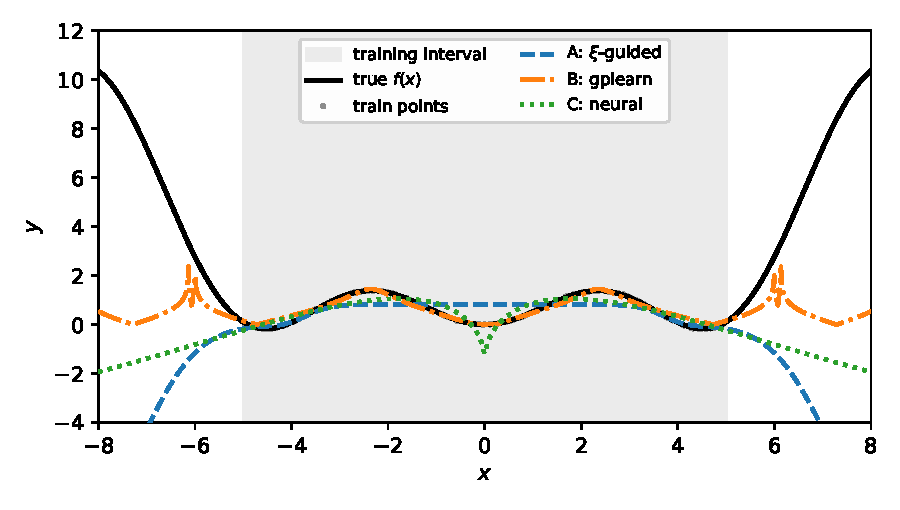
\includegraphics[width=0.85\textwidth]{hero_plot.pdf}
\caption{The hardest test function $0.5\,x\sin x + 0.1x^2$ (black) and
the three regressed functions. Inside the shaded training interval B
tracks the curve closely, while A and C capture the level but not the
oscillation. Outside it, each wrong structure fails in its own way, and
regressor A's prediction contains an unbounded term that leaves the plot
entirely.}
\label{fig:hero}
\end{figure}

\begin{table}[H]
\centering
\begin{tabular}{@{}lrrrrrr@{}}
\toprule
& \multicolumn{3}{c}{NMSE} & \multicolumn{3}{c}{MSE} \\
\cmidrule(lr){2-4} \cmidrule(lr){5-7}
Test band & A & B & C & A & B & C \\
\midrule
1 unit  & 7.4 & 1.1 & 7.0 & 3.6 & 0.5 & 3.5 \\
3 units & 8.8 & 3.1 & 4.9 & 84.9 & 29.6 & 47.8 \\
6 units & 1569.7 & 3.4 & 5.9 & 24562.5 & 53.1 & 92.9 \\
\bottomrule
\end{tabular}
\caption{Errors on $0.5\,x\sin x + 0.1x^2$ as the test band moves
further from the training interval. Raw MSE is given alongside NMSE
because the normalising variance itself grows with the band, by a factor
of $32$ between the first and last row, which makes the NMSE columns
incomparable across rows.}
\label{tab:band}
\end{table}

\subsection{Small training sets}

Finally we fitted $x \sin x$ with strong noise ($0.3$) from only 15, 50
and 200 training points. All methods cope well. Only regressor A shows a
mild effect at $n=15$ (NMSE $0.004$ with a bloated formula instead of
exact recovery), which is expected, since rank statistics such as $\xi$
become unreliable for small $n$. From 50 points on, A and C recover the
exact formula, while B returns the phase-shifted $x \sin(x - 0.028)$ at
$n = 50$ and the exact formula at $n = 200$.

\section{Discussion}

We built a generator for random symbolic functions, three regressors
that return formulas through very different search principles, and a
shared evaluation that scores pure extrapolation. Whenever a method
recovers the true structure, extrapolation is essentially perfect, and
the three fail on complementary targets. A is precise with constants and
robust to noise but cannot assemble sums of several terms, B composes
structures well and even encodes constants as structure but carries a
hard bias on plain numeric coefficients, and C is by far the fastest at
prediction time yet confined to the formulas it saw during pretraining.

The experiments also show the risk that comes with symbolic regression.
A structurally wrong formula can look fine on the training interval and
still explode a few units outside it (Figure~\ref{fig:hero}), and since
in-domain error cannot distinguish a right structure from a similar
wrong one, complexity penalties and validation at some distance from the
training data matter more here than in ordinary regression. An important
note however is that every configuration was run with a single seed, so
differences on any one function carry search variance as well as method
bias, as the non-monotone gplearn values in Section~3.3 show.

Two fixes suggest themselves. The shared failure on
$0.5\,x\sin x + 0.1x^2$ calls for fitting a sparse linear combination of
the best structures a search finds instead of forcing a single winner,
since the $\xi$-guided search already discovers $x\sin x$ and $x^2$
separately but has no way of adding them. Regressor B needs constant
optimisation, but refitting its constants after evolution would help
little, because the bloat is produced during the search itself. The
useful version optimises constants inside the fitness evaluation, which
is what PySR does and \texttt{gplearn} does not offer, and the benchmark
of \citet{lacava2021contemporarysymbolicregressionmethods} finds that
the strongest methods are exactly those combining genetic search with
parameter estimation.

\bibliographystyle{plainnat}
\bibliography{references}
\end{document}